\documentclass[border=10pt]{standalone}
\usepackage{tikz}
\usetikzlibrary{arrows.meta, shapes, calc}

\begin{document}
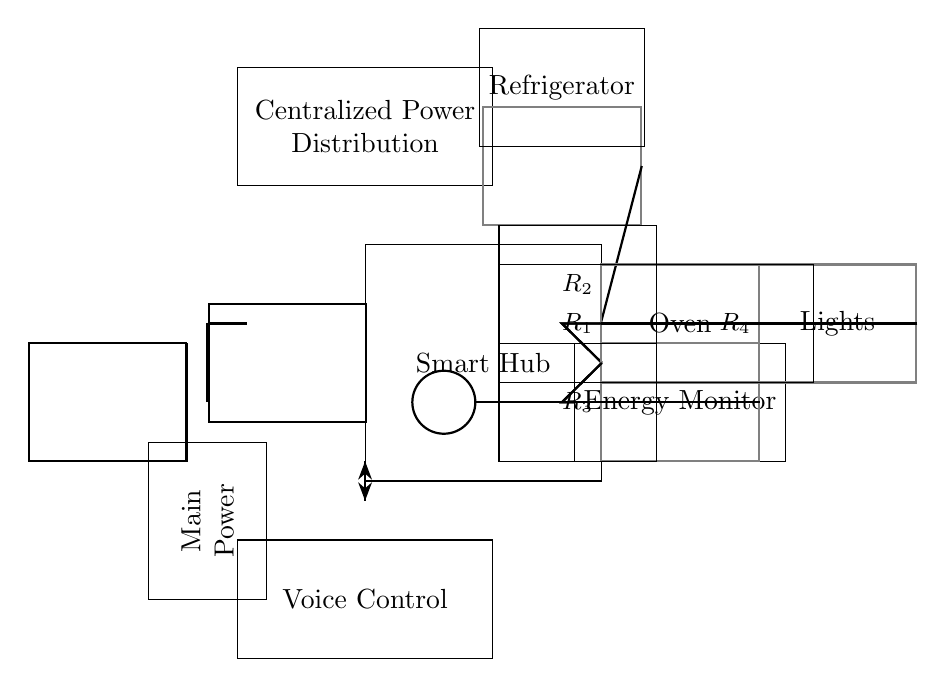
\begin{tikzpicture}[
    node distance=1.5cm,
    every node/.style={draw, minimum width=2cm, minimum height=1.5cm, align=center},
    resistor/.style={thick, gray, rotate=0},
    ammeter/.style={thick, draw, circle, inner sep=0.1cm, minimum size=0.8cm, label={right:}},
    main/.style={thick, black},
    arrow/.style={thick, -Stealth},
    textnode/.style={font=\small}
]

% Main Power
\node (mainpower) [left, text width=1.5cm, align=center, rotate=90] at (0, 0) {Main Power};
\node (battery) [left, draw=none, minimum width=0.5cm, minimum height=1.5cm] at (0, 0.5) {};
\draw[main] (battery.south) -- (battery.north) node[midway, left] {};
\draw[main] (battery.east) -- (0, 0.5) -- (0, 1.5) node[midway, right] {};
\draw[main] (0, 1.5) -- (0.5, 1.5);

% Smart Hub
\node (smart_hub) [right of=battery, minimum width=3cm, minimum height=3cm] at (2, 1) {Smart Hub};

% Centralized Power Distribution
\node (central) [above of=smart_hub, text width=3cm, align=center] at (2, 2.5) {Centralized Power Distribution};

% Voice Control
\node (voice) [below of=smart_hub, text width=3cm, align=center] at (2, -0.5) {Voice Control};
\draw[arrow] (2, -0.25) -- (2, -0.75);
\draw[arrow] (2, -0.75) -- (2, -0.25);

% Energy Monitor
\node (energy_monitor) [right of=smart_hub, minimum width=2cm, minimum height=1.5cm] at (4.5, 0.5) {Energy Monitor};
\node (ammeter) [left of=energy_monitor, ammeter] at (4.5, 0.5) {};
\draw[main] (smart_hub.east) -- (4.5, 0.5) -- (energy_monitor.west);
\draw[main] (ammeter.east) -- (energy_monitor.west);

% Resistor R3
\node (r3) [right of=ammeter, resistor] at (4.5, 0.5) {};
\draw[main] (ammeter.east) -- (r3.west);
\draw[main] (r3.east) -- (energy_monitor.west);

% Oven
\node (oven) [right of=smart_hub, minimum width=2cm, minimum height=1.5cm] at (4.5, 1.5) {Oven};
\node (r2) [above of=oven, resistor] at (4.5, 2) {};
\draw[main] (smart_hub.east) -- (4.5, 1.5) -- (oven.west);
\draw[main] (r2.east) -- (oven.west);

% Refrigerator
\node (refrigerator) [above of=oven, minimum width=2cm, minimum height=1.5cm] at (4.5, 3) {Refrigerator};

% Lights
\node (lights) [right of=oven, minimum width=2cm, minimum height=1.5cm] at (6.5, 1.5) {Lights};
\node (r4) [right of=oven, resistor] at (6.5, 1.5) {};
\draw[main] (oven.east) -- (6.5, 1.5) -- (lights.west);
\draw[main] (r4.east) -- (lights.west);

% Resistor R1
\node (r1) [right of=smart_hub, resistor] at (4.5, 1.5) {};
\draw[main] (smart_hub.east) -- (4.5, 1.5) -- (oven.west);
\draw[main] (r1.east) -- (oven.west);

% Resistor R3 (again, for clarity)
\node (r3_again) [right of=smart_hub, resistor] at (4.5, 0.5) {};
\draw[main] (smart_hub.east) -- (4.5, 0.5) -- (energy_monitor.west);
\draw[main] (r3_again.east) -- (energy_monitor.west);

% Labels for resistors
\node[textnode] at (4.7, 2) {$R_2$};
\node[textnode] at (4.7, 1.5) {$R_1$};
\node[textnode] at (4.7, 0.5) {$R_3$};
\node[textnode] at (6.7, 1.5) {$R_4$};

\end{tikzpicture}
\end{document}